
\section{Research Design}
\label{design}


\subsection{Models}

This project will assess the viability of using Bayesian Gaussian Process models for spatiotemporal predictions in urban settings. Gaussian Processes have attractive properties for sparse data because a model can be interpreted as interpolating an unobserved point between known distributions \todo{Also, not totally confident in this statement}. As mentioned in the literature review, spatiotemporal models have historically suffered from computational infeasibility when the amount of data as well as spatial and temporal dimensionality grows. Recent advances in Bayesian probablistic programming (Stan) and implementations of Gaussian Processes that take advantage of the relative sparsity of data across spatial dimensions has reduced the computational burden of fitting these models, although the spatial granularity proposed here will require a great deal of posterior checks to ensure the model is fitting correctly. \par

A Gaussian Process model will be compared to  existing spatial, temporal, and spatiotemporal modeling methods for this type of forecasting problem. Standard maximum-likelihood autoregressive models like ARIMA will be considered, as well as existing Bayesian methodologies like INLA. Out-of-sample predictive accuracy will be assessed with a root-mean-squared-error (RMSE) metric that
can be easily applied to all models. Robustness of forecasting results and model sensitivity to tuning parameters will also be assessed with the goal of providing insight into the practical viability of running models in a production environment. The relative speed of fitting different models will also be a factor for assessing viability. \par

\subsection{Gaussian Processes}

\subsection{The Log-Gaussian Cox Process}

Log-Gaussian Cox Process (LGCP) models are a further extension of a Gaussian Process with particular applicability to prediction of count data. A LGCP is hierarchical in that the data are assumed to be drawn from a Poisson likelihood with intensity parameter $\lambda$. The Poisson likelihood function has theoretical properties suitable for relatively sparse count (integer) data which makes it appealing for use in modelling frequent events that are nevertheless sparse when segmented over space and time dimensions. In turn the log of $\lambda$  is generated by a Guassian process\cite{teng_2017}. This makes the LGCP quite flexible in inputs and dimensionality while also making model fitting generally computationally burdensome. \par

An alternative specification used a Gaussian likelihood, which has the added appeal of making the likelihood and prior conjugate to each other and solvable in closed form. As the $\lambda$ parameter of a Poisson distribution increases the distribution converges to a Normal distribution anyway, so this model may be more applicable to situations when counts are not sparse e.g., at lower granularities of space and/or time, which was not considered in detail here \todo{ADD SOME DATA for normal model?}.

A zero-inflated Binomial (ZIB) likelihood would be another alternative to consider for this type of modelling. As the name implies, a ZIB distribution has a higher probability density around zero and may be better suited for extremely sparse data like gridded observations with very small grid dimensions.

 The general model follows the specification and notation used by "A General Approach to Prediction and Forecasting Crime Rates with Gaussian Processes" \cite{flaxman_2014}: \par


$$\lambda(s,t) = exp((s,t))$$

$$ y_{s,t} | \lambda(s,t) ~ Poisson(exp(f(s,t))e_t) $$

The outcome count $y_{s,t}$ at location $s$ and time $t$ is generated from a Poisson distribution with parameter $f(s,t)e_t$. $f(s,t)$ is a function with a Gaussian process prior, while $e_s$ is a fixed spatial expectation term $\mathbb{E}[y_s]$. The spatial expectation is a convenient way to incorporate prior information about the variable of interest. Again following Flaxman 2014, using an exponential link function gives a practical interpretation of $exp(f(s,t))$ as the relative risk function while $f(s,t)$ itself is the log-relative risk. When the log-relative risk is 0, the relative risk is 1 and the expected value of of the outcome $y(s,t)$ is just the prior spatial expectation $e_s$. Finally, every count outcome $y_{s,t}$ is assumed independent conditional on $f$, so the joint conditional likelihood of all $y$ factors as a product.

$$p(y|f) = \prod{ Poisson(exp(f(s,t))e_t)}$$

\subsubsection{f(s,t)}

$f$ is modeled as following a generic Gaussian process with a mean of zero and a covariance matrix $K$:

$$ f ~ GP(0,K) $$

Spatiotemporal elements enter the Gaussian process model through $K$, which is used to capture the relationships of interest and entirely determines the model. Since variance/covariance is additive, any variance term can be decomposed at least theoretically into arbitrarily many additive components. Purely spatial and temporal elements as well as interactions can be incorporated using different kernel functions, and different combinations of kernels may produce more accurate results. Cross-validating models with different types and combinations of kernel functions will help identify the specification with the best predictive properties. Since the cross-validation data are correlated in this model the cross-validation set will have to be drawn from spatially contigous representative subsets of the data.

\subsubsection{Kernels}

There are a wide variety of existing kernel functions documented for use in Gaussian process models \cite{rasmussen_2005} and it is also possible to define custom functions as long as they follow certain properties. Since the entire model is determined by its kernels there is a lot of room for experimentation and choice. \par

An important consideration is whether the model is considered to be stationary. In spatiotemporal models the case for assuming stationarity weakens as the time-period being considered lengthens, and this should in turn affect the kernel choice. The long term model considered includes a non-stationary linear kernel component intended to capture any long-term trends:    \par

\begin{itemize}
  \item $k_t(t)$ : a temporal kernel
  \item $k_p(t)$ : a periodic kernel
  \item $k_l$: a linear kernel
\end{itemize}

The short-term models considered for this project are all stationary and loosely follow Flaxman 2014 by consisting of up to four individual kernels $k$ , where $K=\sum{i}k_i$. The four basic kernel types were:

\begin{itemize}
  \item $k_s(s)$ : a spatial kernel
  \item $k_t(t)$ : a temporal kernel
  \item $k_p(t)$ : a periodic kernel
  \item $k_{st}(s,t)$ : a space-time interaction kernel
\end{itemize}

The kernel types specified for each $k$ differed slightly from Flaxman after experimenting with various configurations. Both a squared exponential and Matern-32 kernel were considered for the spatial component.

\todo{stationary vs. non-stationary}
\todo{kernel plots (Matern vs. RBF?)}


\subsubsection{Priors}

Gelman 2006 suggests using a student-t prior distribution restricted to be positive (a 'half-t') as a prior for variance parameters in hierarchical models \cite{gelman_2006}. Since variance is always positive it is acceptable and desirable to restrict the prior distribution to be non-negative as well. Flaxman 2014 used a standard student-t prior with 4 degrees of freedom on all parameters (not just variance). The GPflow package doesn't currently offer a student-t prior of any kind, so a normal distribution was used as a substitute. The normal prior has less probability mass in its tails than the Student-t but is otherwise a close substitute. A standard $N~(0,1)$ was used for all but the spatial kernel $k_s(s)$, which had a $N~(0,5)$ prior. This was necessary as the smaller $\sigma$ value sometimes caused the optimization algorithm to fail.

\subsubsection{Methods for fitting LGCPs}

Solutions to the computational challenges in fitting LGCPs have advanced rapidly over the past five years. The computational bottleneck for Gaussian Process models is the the n-by-b covariance matrix, which requires an $O(n^3)$ computation. Fitting a GP model as $n$ grows beyond a few thousand points is quite challenging \cite{gelman2013bayesian}. \par

 As recently as 2012 the best methods for fitting LGCP models involved variations of the Metropolis-Hastings sampling algorithm which were considered to be slow and highly inefficient in generating acceptable draws from the posterior distribution of the model \cite{murray_2012}. Advances in statistical computing have opened the door for several new model fitting methods, each with their own advantages and drawbacks.

\subsubsection{Variational Inference}

Variational Inference (VI) methods attempt to recover parameter estimates for a posterior distribution of interest by specifying a more tractable family of distributions and optimizing the resulting approximation using closed-form or computational methods. In the case of the LGCP there is no direct closed-form solution, but advances in computation - in particular autodifferentiation algorithms - have made the process easier. However, there are no theoretical justifications for the accuracy of estimates produced by VI because it is unclear and often unknowable how close the optimized approximation is to the true posterior distribution (Kullback-Leibler divergence). Yao et., al. recently proposed several diagnostic methods for assessing whether a VI approximation actually 'worked' \cite{yao_2018}.

\subsubsection{MCMC}

Markov Chain Monte Carlo (MCMC) sampling methods by contrast do have theoretical properties that ensure consistent estimation of the posterior distribution - at least  as the numbers of samples increases asympotically \cite{teng_2017}. MCMC methods are not a new development in themselves, but there have been breakthroughs both in MCMC algorithm design and computing power required to fit more complex models. Stan has been used for spatiotemporal modelling of causes of mortality using Gaussian Markov Random Field models, another potential alternative to LGCPs that may be appropriate for urban forecasting but are not considered here \cite{foreman_2017}. In contrast to VI, MCMC also is capable of producing estimates for full posterior distributions for parameters of interest, rather than point estimate approximations. In the case of urban prediction and forecasting, access to full posterior estimates would offer much more probalistic information from which to draw uncertainty-based conclusions in a policy or administrative context \todo{EXAMPLE HERE}.

\subsubsection{VFF}
\todo{MAYBE MOVE TO DISCUSSION, add mention Kronecker methods}

see GPML pg. 82 , Bohner's theorem


\subsubsection{Method Choice}

While MCMC methods clearly offer desirable properties superior to VI methods, their practical limitations made them somewhat burdensome to consider for this project. The most unfortunate drawbacks were that MCMC is very slow to fit in comparison with VI and that specifying tractable LGCP models in an MCMC language such as Stan requires writing more complex and less flexible code \cite{Flaxman2015FastHG}. In an attempt to draw a compromise between ease of experimentation and model reliability this project used primarily VI methods under the knowledge that these methods may not produce the best results for practical use.



\subsection{Model Specification}


\subsection{Data}

This project will use observational administrative data gathered as part of New York City's Open Data civic reporting system. There are many recorded urban events outside of the aforemented policing context where predictive and forecasting knowledge could be helpful to resarch, policy, or operations. Quality-of-life programs such as noise abatement, pest control, and traffic reduction are all natural candidates where data is already collected from the public; in New York City it is done through the 311 civil reporting system. Each also involves allocating scarce public resources e.g., public safety officers, exterminators, and health inspectors over space and time. \par

Although the aforementioned urban events are ex-ante all topic of interests with some potential for spatiotemporal forecastability and would benefit from more accurate modelling, this project instead focused on another heavily spatially dependent public safety issue: vehicle collisions. There have been over 200 fatalities annually resulting from vehicle collisions in New York City over the past five years while Mayor Bill de Blasio's Vision Zero plan has publicly stated a goal of lowering the number of fatalities to zero \cite{nyc_vz}. \par

While approximately 200 fatalities a year is not a 'rare' event, the likelihood of observing a fatality at any given time and place in New York City is exceedingly rare. What's more, public safety interventions in the form of increased enforcement or street redesign can be deployed reactively to the scene of a fatality with little or no information about the true relative risk of that location \todo{can I cite Jonathan here?}. \par

By contrast, non-fatal injuries resulting from traffic collisions are much more common, with X in 2017 alone where Y of them were marked as serious \todo{fill in injury stats}. By thinking of injuries as a potential fatality observing and attempting to forecast these injures reliably could provide a much better estimate of where the city is particularly risky for traffic collisions. These estimates could in turn be used to evaluate the efficacy of any public safety intervention after the fact instead of relying on observing only the future fatality count which may be subject to mean reversion in a situation where the mean fatalities at any given place and time are very close to zero.

\subsubsection{Data Processing}

Organizing spatiotemporal count data into a suitable form for modelling presents a challenge in itself. While every count observation occured at a specific point and time, aggregating to a form appropriate both for modelling and capable of providing useful granular forecasts is a balancing act. Traffic collisions in particular are difficult to aggregate into consisten spatial locations that also have a coherent interpretation of the distance between each location necessary for fitting a spatiotemporal model. \par

There are many administrative spatial aggregation bounds which are of potential use, such as Neighborhoods, Zip Codes, Census Blocks, or even unique street intersection IDs. While all may be perfectly viable depending on the situation, gridding provides a more generalizable spatial aggregation method which is already used in many spatial statistics applications, see for example the case studies in \cite{blangiardo_2015}. Gridding simply overlays a square grid of chosen size on the area of interest and sums all the count data within each grid cell into a single data point, a flexible method that can be easily - if imperfectly - applied to many spatial contexts. Being able to flexibly choose the size of grid squares adds an additional layer of modelling flexibility. \par

\todo{NTA summarization: plot of NTA centroids in MN.}

Finally gridding offers clear benefits in the specific case of Gaussian process models. Since the spatial kernel $k_s$ calculates the distance between any point $s_i$ and all other points in $s$ the computational cost of adding an additional point in $s$ is high and a GP model runs in $\mathbb{O}(n^3)$  \cite{flaxman_2015_FastKron}. By specifying the distance calculation only between the centroid of each grid square this method at least offers an explicit choice between higher spatial resolution and computational complexity.

\begin{figure}[h!]
  \caption{A grid of 1250ft grid squares overlaid on the Park Slope street grid.}
  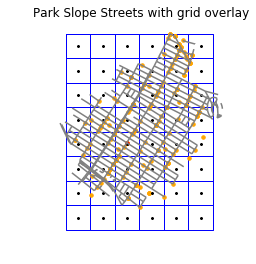
\includegraphics[width=0.5\textwidth]{PS_street_grid}
\end{figure}
